\documentclass[conference]{IEEEtran}
% \IEEEoverridecommandlockouts
% The preceding line is only needed to identify funding in the first footnote. If that is unneeded, please comment it out.
\usepackage{cite}
% \usepackage{amsmath,amssymb,amsfonts}
\usepackage{amsmath}% equation formatting
% \usepackage{algorithmic}% Algorithms
\usepackage{graphicx}
\graphicspath{{img/}}
% \usepackage{textcomp}% Text Companion fonts
\usepackage[usenames,dvipsnames]{xcolor}
\def\BibTeX{{\rm B\kern-.05em{\sc i\kern-.025em b}\kern-.08em
    T\kern-.1667em\lower.7ex\hbox{E}\kern-.125emX}}

\usepackage[cmintegrals]{newtxmath}% equation font similar to the rest
\usepackage{microtype}
\usepackage[T1]{fontenc} %set the font (output) encoding
% \usepackage[brazil]{babel} %"sumário", "capítulo", etc.
\usepackage{hyphenat}
% \hyphenation{mate-mática recu-perar}
\usepackage{cite}
\usepackage{booktabs}
\usepackage{listings}
\makeatletter
\let\@ORGmakecaption\@makecaption
\long\def\@makecaption#1#2{\@ORGmakecaption{#1}{#2}\vskip\belowcaptionskip\relax}
\makeatother
\lstdefinestyle{mystyle}{
frame               = single,
rulecolor           = \color{gray},
basicstyle          = \ttfamily\scriptsize,
belowcaptionskip    = 8pt,
aboveskip           = 8pt,
belowskip           = 8pt,
columns             = fullflexible,
breakatwhitespace   = false,
breaklines          = true,
keepspaces          = true,
showspaces          = false,
showstringspaces    = false,
inputencoding       = utf8,
extendedchars       = true,
literate            =
{á}{{\'a}}1 {é}{{\'e}}1 {í}{{\'i}}1 {ó}{{\'o}}1 {ú}{{\'u}}1
{Á}{{\'A}}1 {É}{{\'E}}1 {Í}{{\'I}}1 {Ó}{{\'O}}1 {Ú}{{\'U}}1
{à}{{\`a}}1 {è}{{\`e}}1 {ì}{{\`i}}1 {ò}{{\`o}}1 {ù}{{\`u}}1
{À}{{\`A}}1 {È}{{\'E}}1 {Ì}{{\`I}}1 {Ò}{{\`O}}1 {Ù}{{\`U}}1
{ä}{{\"a}}1 {ë}{{\"e}}1 {ï}{{\"i}}1 {ö}{{\"o}}1 {ü}{{\"u}}1
{Ä}{{\"A}}1 {Ë}{{\"E}}1 {Ï}{{\"I}}1 {Ö}{{\"O}}1 {Ü}{{\"U}}1
{â}{{\^a}}1 {ê}{{\^e}}1 {î}{{\^i}}1 {ô}{{\^o}}1 {û}{{\^u}}1
{Â}{{\^A}}1 {Ê}{{\^E}}1 {Î}{{\^I}}1 {Ô}{{\^O}}1 {Û}{{\^U}}1
{œ}{{\oe}}1 {Œ}{{\OE}}1 {æ}{{\ae}}1 {Æ}{{\AE}}1 {ß}{{\ss}}1
{ç}{{\c c}}1 {Ç}{{\c C}}1 {ø}{{\o}}1 {å}{{\r a}}1 {Å}{{\r A}}1
{€}{{\EUR}}1 {£}{{\pounds}}1 {ã}{{\~a}}1 {Ã}{{\~A}}1,
showtabs=false,
tabsize=2,
}
\lstset{}
\lstset{style=mystyle}

\usepackage{xurl}
\usepackage[colorlinks,urlcolor=blue]{hyperref}
\renewcommand{\figureautorefname}{Fig.}%
% \renewcommand{\tableautorefname}{Tabela}%
% \renewcommand{\equationautorefname}{Equação}%
% \renewcommand{\lstlistingname}{Listagem}%

\usepackage{placeins}% \FloatBarrier
\usepackage[bottom]{footmisc}% \footnote
%\setlength{\skip\footins}{.5cm}

\usepackage{lipsum}

%----------------------------------------
% user defined commands
%----------------------------------------
\newcommand{\F}[1]{\footnote{\url{#1}}}



%========================================
\begin{document}
%========================================

\title{Solution of a One-Dimensional Viscous Burgers' Equation Using a Physics-Informed Neural Network and a Gaussian Quadrature Method
%\\
% {\footnotesize \textsuperscript{*}Note: Sub-titles are not captured in Xplore and
% should not be used}
% \thanks{Identify applicable funding agency here. If none, delete this.}
}

\author{\IEEEauthorblockN{Eduardo F. Miranda}
\IEEEauthorblockA{
% \textit{dept. name of organization (of Aff.)} \\
% \textit{name of organization (of Aff.)}\\
% City, Country \\
eduardofurlanm@gmail.com}
% \and
% \IEEEauthorblockN{2\textsuperscript{nd} Given Name Surname}
% \IEEEauthorblockA{\textit{dept. name of organization (of Aff.)} \\
% \textit{name of organization (of Aff.)}\\
% City, Country \\
% email address or ORCID}
% \and
% \IEEEauthorblockN{3\textsuperscript{rd} Given Name Surname}
% \IEEEauthorblockA{\textit{dept. name of organization (of Aff.)} \\
% \textit{name of organization (of Aff.)}\\
% City, Country \\
% email address or ORCID}
% \and
% \IEEEauthorblockN{4\textsuperscript{th} Given Name Surname}
% \IEEEauthorblockA{\textit{dept. name of organization (of Aff.)} \\
% \textit{name of organization (of Aff.)}\\
% City, Country \\
% email address or ORCID}
% \and
% \IEEEauthorblockN{5\textsuperscript{th} Given Name Surname}
% \IEEEauthorblockA{\textit{dept. name of organization (of Aff.)} \\
% \textit{name of organization (of Aff.)}\\
% City, Country \\
% email address or ORCID}
% \and
% \IEEEauthorblockN{6\textsuperscript{th} Given Name Surname}
% \IEEEauthorblockA{\textit{dept. name of organization (of Aff.)} \\
% \textit{name of organization (of Aff.)}\\
% City, Country \\
% email address or ORCID}
}

\maketitle
% page numbering:
\thispagestyle{plain}
\pagestyle{plain}

\begin{abstract}
% Abstract revisado, novo
This work compares the solutions of a one-dimensional viscous Burgers’ equation of a test problem using a Physics Informed Neural Network (PINN) and a numerical Gaussian Quadrature Method (GQM) method. The Burgers' equation is a partial differential equation (PDE) with derivatives in both space and time, which is commonly solved by a numerical method. However, recent works have proposed the solution by means of Artificial Neural Networks (ANNs). Since the number of sample/collocation points (in space and time) required for an efficient training of the ANN would be too high, PINNs were proposed to allow the use of less sample points by embedding the related equation of physics into the simulation. This work compares the solutions of the one-dimensional viscosity Burgers' equation for a test problem obtained by the PINN and by the GQM methods. Accuracy and required processing time of the solutions, both executed in the LNCC Santos Dumont supercomputer, are also presented.
\end{abstract}

% \begin{IEEEkeywords}
% component, formatting, style, styling, insert
% \end{IEEEkeywords}

%
%
%
%----------------------------------------
\section{Introduction}
%----------------------------------------
%
Many simulations are mathematically modeled by partial differential equations (PDEs), which have derivatives in space and time. However, the coefficients of these derivatives are unknowns, and the PDEs are usually solved by a numerical method, like the Finite Difference Method (FDM) or the numerical Gaussian Quadrature Method (GQM). Recent works proposed to solve PDEs using Artificial Neural Networks (ANN), which are Machine Learning (ML) algorithms. The universal approximation theorem states that a neural network can approximate any continuous function, provided the network has a sufficient number of hidden layer and that employs non-linear activation functions. This approach requires to know a large set of sample points in space and time in order to perform the training of the neural network, and such sample points are named Collocation Points (CPs).
Since the required number of CPs would be too high, Physics Informed Neural Networks (PINNs) were proposed to allow the use of less CPs by including in the ANN the underlying physical laws related to the simulation.   

This work compares the solutions of the viscous Burgers equation, a PDE with derivatives in both space and time, for a test problem, by a PINN and a GQM. This equation models the velocity of a viscous fluid, being a particular case of the Burgers equation for fluid mechanics. The corresponding PINN and GQM solutions%
\footnote{The code is available at \url{https://github.com/efurlanm/421/tree/main/project}}
are compared in terms of accuracy and processing time, both executed in the Santos Dumont supercomputer. Tests were executed in a Bull B710 processing node of the supercomputer Santos Dumont of the LNCC (National Laboratory of Scientific Computing). It has two Intel Xeon E5-2695v2 Ivy Bridge 2.4 GHz 12-core processors (total of 24 cores), and 64 GB of main memory.

The solution of PDEs by PINNs is relatively recent and acquiring knowledge in such approach may be useful for solving PDEs in some specific modules of numerical models used at CPTEC/INPE for weather and climate forecast. 
%
%----------------------------------------
\section{Material and methods}\label{sec:meth}
%----------------------------------------
%
Raissi et al. (2019) \cite{Raissi2019} published an article about PINNs, which has 4152 citations. That work defines PINNs as ANNs trained to solve supervised learning tasks, but complying to physical laws, usually described by nonlinear PDEs. It also describes the use of ANNs to solve PDEs and obtain physics-informed surrogates of the physical model that are fully differentiable in all coordinates and free parameters. PINNs form a new class of data-efficient universal function approximators, which can be effectively trained using small datasets, and which may encode any underlying physical law. 

Unlike standard numerical methods, the PINN solution can be obtained without specifying the spatial or temporal domain discretization. The training data is randomly sampled from simulations using synthetic data obtained using a known equation, or randomly generated, or even from observational data. This sampled data contains points in the space and time domain called collocation points (CPs). Except for the randomly generate data, provided that a sufficient number of CPs is available, a standard ANN may solve the PDE, otherwise a PINN would be required. A PINN uses a specific loss function in the training phase that embeds the applicable physical law and is calculated from the set of CPs and, eventually, also the ICs and BCs \cite{Cuomo2022}.

PINNs can be considered neural networks for supervised learning problems, as proposed here. However, PINNs can also be used as agents for reinforcement learning (RL) \cite{Cuomo2022}. The most common PINN architectures are Multi-layer Perceptrons (MLPs), Convolutional Neural Networks (CNNs) and Recurrent Neural Networks (RNNs). Newer architectures are Auto-Encoder (AE), Deep Belief Network (DBN), Generative Adversarial Network (GAN) and Bayesian Deep Learning (BDL) \cite{Cuomo2022}. 

The proposed test case requires the solution of a particular one-dimensional viscous Burger equation with Dirichlet boundary condition (BC) and initial condition (IC), which estimates the velocity field $u$ along time (\autoref {eq:burg}). Training data for the PINN is given by a set of CPs corresponding to the velocity field in different times are randomly generated within the considered domain.
 
In the train phase, the network then estimates a solution $u(t,x)$. 
The function employed by the PINN $f(t,x)$ (\autoref {eq:ftx}) is derived from the known viscous Burgers equation, and allows to calculate the loss function.  
%and implemented using Python and the library TensorFlow. 
In the following equations, $u$ is the velocity, the coefficient ${(100\pi)}^{-1}$ is the kinematic viscosity, and the subscripts denote partial differentiation in time and space, respectively, as
$u_t$ (which denotes $\frac{du}{dt}$), 
$u_x$ (which denotes $\frac{du}{dx}$), and 
$u_{xx}$ (which denotes $\frac{d^2u}{dx^2}$).

\begin{flalign}\label{eq:burg}
&u_t + uu_x - {(100\pi)}^{-1}u_{xx} = 0, \quad x \in [-1,1], \ t \in [0, 1],\\
\nonumber &u(0, x) = - sen(\pi x), \quad \ \ \text{(IC)}\\
\nonumber &u(t, -1) = u(t, 1) = 0. \quad \text{(BC)}
\end{flalign}

The viscous Burguers equation is employed to evaluate the error $f$ of the solution $u(t,x)$ estimated by the PINN, as shown in \autoref {eq:ftx}.

\begin{equation}\label{eq:ftx}
f := u_t + uu_x - {(100\pi)}^{-1}u_{xx}
\end{equation}

In this work, the PINN loss function to be minimized is given by the mean squared error (\autoref {eq:mse}) of two components, $MSE_u$, which embeds the error considering ICs and BCs, and $MSE_f$, which embeds the errors considering the set of CPs, where $t$ is the time step, and $x$ is the one-dimension coordinate. 

\begin{equation}\label{eq:mse}
MSE = MSE_u + MSE_f
\end{equation}
where
$$ MSE_u = \frac{1}{N_u}\sum_{i=1}^{N_u}|u(t^i, x^i)-u^i|^2  \quad \text{(IC and BC)}$$
and
$$ MSE_f = \frac{1}{N_{CP}}\sum_{i=1}^{N_{CP}}|f(t^i, x^i)|^2  \quad \text{(CP)}$$

% ----------------------------------------
\subsection{Numerical GQM Implementation of the Test Problem}
% ----------------------------------------

A Fortran 90 implementation of the GQM method was used to generate the full dataset of the velocity field, which was taken as reference solution in the comparison with the PINN solution.
 The GQM dataset has 100 time steps in the interval [0, 99] and 256 one-dimensional grid points in the interval [-1, 1], defining a velocity field $u(x,t)$ subjected to the ICs and BCs shown in \autoref {eq:burg}. 
%A number of $N_f=10,000$ points we randomly sampled from this dataset as CPs.

The GQM method is an iterative numerical algorithm that approximates the definite integral of a function as a weighted sum of the function values at specified points within the domain of integration \cite{Burkardt2013}. The order of quadrature rule was set to 8. The loops corresponding to the compute-intensive part of the code were parallelized with the OpenMP 3.1 library using the \lstinline{!$OMP PARALLEL DO$} directive, since there is no data dependency between loop iterations. The F90 code was compiled with GNU 4.8.5 setting the -O3 optimization flag. The code was also executed using CPU cores with 1, 4, 8, 16 and 24 OpenMP threads.   

% ----------------------------------------
\subsection{PINN Implementation of the Test Problem}
% ----------------------------------------

The particular architecture of the PINN implemented in this work is a feed-forward MLP with a 2-neuron input layer, eight 20-neuron hidden layers, and a single-neuron output layer. The loss function is the Mean Square Error (MSE). The minimization of the loss function is performed by an optimization method like the widespread Limited-memory BFGS (L-BFGS) algorithm, a quasi-Newton method that approximates the Broyden–Fletcher–Goldfarb–Shanno algorithm (BFGS). All hidden layers employ the hyperbolic tangent as the activation function.

The PINN implementation was based on the work of Raissi et al. (2019) \cite{Raissi2019} and uses 
the TensorFlow\F{http://www.tensorflow.org} 1.15 library and the Python 3.7 interpreter. Code snippets of the TensorFlow library are shown in \autoref {lst:utx} and \autoref {lst:ftx}. Note that the snippets do not show the implementation of the BCs, ICs and other details. The code was also executed using CPU cores Tests with 1, 4, 8, 16 and 24 OpenMP threads.   

\begin{lstlisting}[language=Python, label=lst:utx, caption={Code snippet that implements $u(t,x)$}]
def u(t, x):
    u = neural_net(tf.concat([t, x], 1), weights, biases)
    return u
\end{lstlisting}

\begin{lstlisting}[language=Python, label=lst:ftx, caption={Code snippet that implements $f(t,x)$}]
def f(t, x):
    u = u(t, x)
    u_t = tf.gradients(u, t)[0]
    u_x = tf.gradients(u, x)[0]
    u_xx = tf.gradients(u_x, x)[0]
    f = u_t + u*u_x - (0.01/tf.pi)*u_xx
    return f
\end{lstlisting}

%
%----------------------------------------
\section{Results}\label{sec:resu}
%----------------------------------------
% Analysis of the Parallel Performance for the Test Problem

The PINN solution $u(t,x)$ is shown in \autoref{fig:bur1}, with the time $t$ in the horizontal axis  and the spatial coordinate $x$ in the vertical axis. The red marks in the boundaries of the graph represent the 100 randomly assigned points (BC+IC) used for training. The 10,000 CPs randomly generated are not shown. The color scale refers to the velocity $u(x,t)$. The dashed vertical lines refer to 2 specific snapshots ($t=0.25$ and $t=0.75$). \autoref {fig:bur2} shows the superimposed solutions for PINN and GQM for these 2 snapshots, which are quite equivalent.

\begin{figure}[htb]
\centering
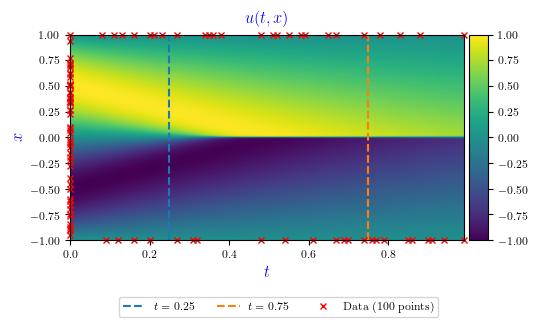
\includegraphics[width=\linewidth]{burgers01}
\caption{PINN solution for the velocity $u(t,x)$. The horizontal axis denotes time $t$, and the vertical axis, the coordinate $x$. The red marks in the boundaries of the graph represent the 100 randomly assigned points (BC+IC) used for training. The color scale refers to the velocity. The dashed vertical lines refer to 2 snapshots ($t=0.25$ and $t=0.75$).} 
\label{fig:bur1}
\end{figure}


\begin{figure}[htb]
\centering
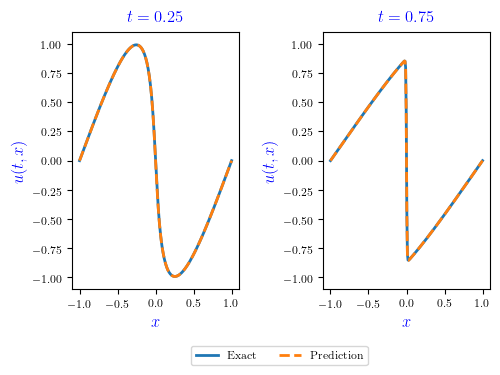
\includegraphics[width=.9\linewidth]{burgers02}
\caption{Superimposed solutions for PINN and GQM for the $t=0.25$ and $t=0.75$ snapshots. PINN solution is labeled as \textbf{Prediction}, \textcolor{orange}{in orange}), and GQM solution is labeled as \textbf{Exact}, \textcolor{NavyBlue}{in blue}).}
\label{fig:bur2}
\end{figure}

\begin{table}[htb]
\centering
\caption{Processing times, speedups and parallel efficiencies for the PINN and GQM solutions for different numbers of OpenMP threads. The GQM single-thread execution time was taken as a reference, highlighted in blue. Best values are highlighted in red.}
\label{tab:resu}
% a tabela está no Google Docs: https://docs.google.com/spreadsheets/d/1yQdTPwtr5UYZEvoaSrflA00kdqxVqdQP4wzRpYuj-EM/edit?usp=sharing
% depois de alterada, basta copiar para o arquivo tab_resu.tex
\begin{tabular}{lrrrrr}\toprule											
	&	\multicolumn{5}{c}{\textbf{Number of OpenMP threads}}									\\
\cline{2-6}\vspace{-8pt}	&		&		&		&		&		\\
\textbf{Profiling}	&	\textbf{1}	&	\textbf{4}	&	\textbf{8}	&	\textbf{16}	&	\textbf{24}	\vspace{1pt}\\
\toprule\vspace{-10pt}	&		&		&		&		&		\\
\multicolumn{6}{c}{\textbf{\textit{Processing time (seconds)}}}											\\
\midrule[0.1pt]\vspace{-10pt}	&		&		&		&		&		\\
\textbf{GQM}	&	\color{blue}{0.02}	&	\color{red}{0.01}	&	\color{red}{0.00}	&	\color{red}{0.00}	&	\color{red}{0.00}	\\
\textbf{Train}	&	30.33	&	22.14	&	21.69	&	22.56	&	23.21	\\
\textbf{Predict}	&	0.10	&	0.05	&	0.03	&	0.03	&	0.03	\\
\toprule\vspace{-10pt}	&		&		&		&		&		\\
\multicolumn{6}{c}{\textbf{\textit{Speedup}}}											\\
\midrule[0.1pt]\vspace{-10pt}	&		&		&		&		&		\\
\textbf{GQM}	&	\color{blue}{1.00}	&	\color{red}{3.11}	&	\color{red}{5.39}	&	\color{red}{7.43}	&	\color{red}{9.77}	\\
\textbf{Train}	&	0.00	&	0.00	&	0.00	&	0.00	&	0.00	\\
\textbf{Predict}	&	0.20	&	0.43	&	0.63	&	0.71	&	0.73	\\
\toprule\vspace{-10pt}	&		&		&		&		&		\\
\multicolumn{6}{c}{\textbf{\textit{Parallel efficiency}}}											\\
\midrule[0.1pt]\vspace{-10pt}	&		&		&		&		&		\\
\textbf{GQM}	&	\color{blue}{1.00}	&	\color{red}{0.78}	&	\color{red}{0.67}	&	\color{red}{0.46}	&	\color{red}{0.41}	\\
\textbf{Train}	&	0.00	&	0.00	&	0.00	&	0.00	&	0.00	\\
\textbf{Predict}	&	0.20	&	0.11	&	0.08	&	0.04	&	0.03	\\
\bottomrule											
\end{tabular}											
\end{table}

\begin{figure}[htb]
\centering
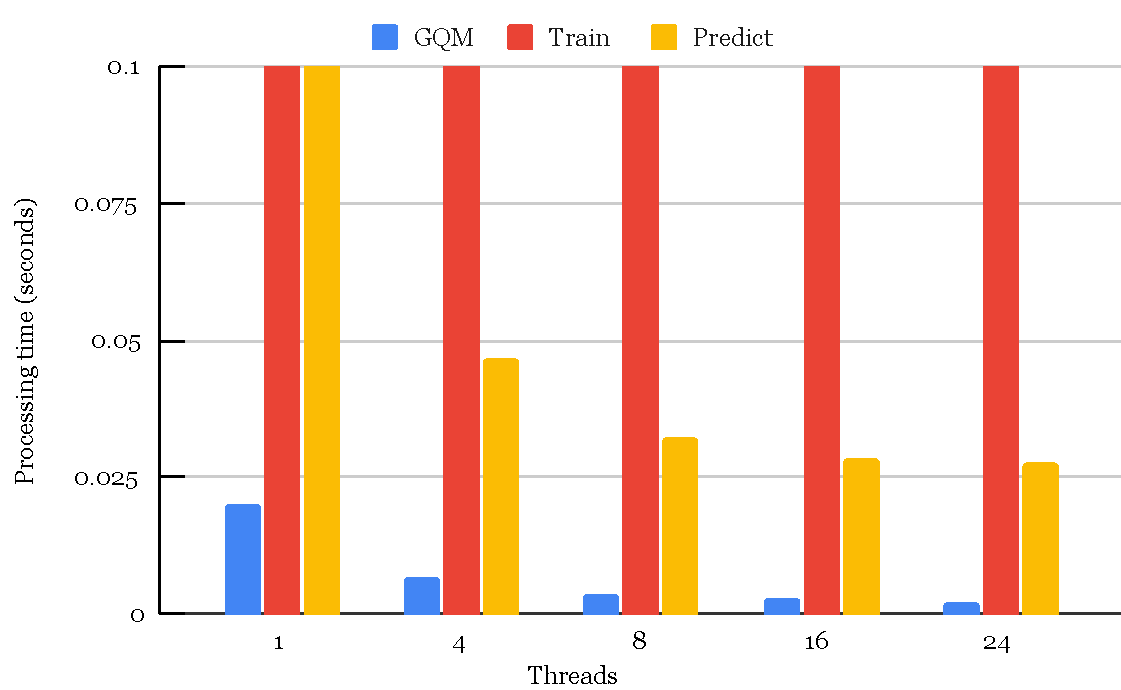
\includegraphics[width=\linewidth]{resu_time}
\caption{Processing times (seconds) in function of number of OpenMP threads for the GQM and PINN implementations. "Train" refer to the PINN training phase, while "Predict" refers to the PINN test/prediction phase (for convenience, times above 0.1 seconds are not shown).}
\label{fig:time}
\end{figure}

\begin{figure}[htb]
\centering
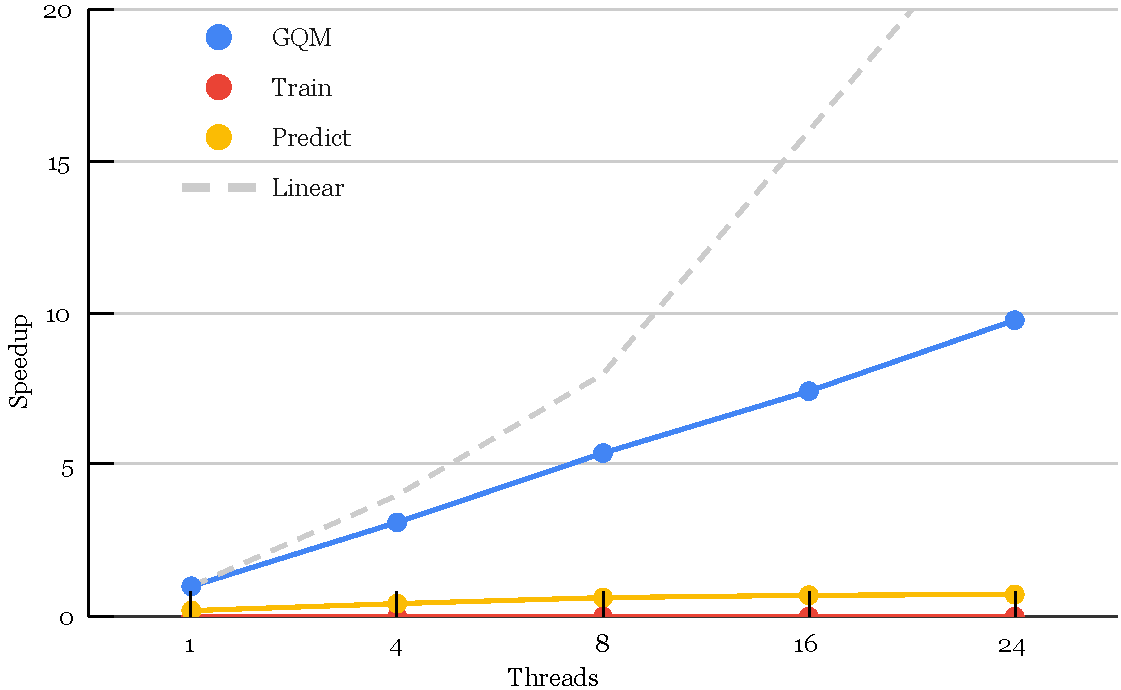
\includegraphics[width=\linewidth]{resu_spee}
\caption{Speedups in function of the number of OpenMP threads for the GQM and PINN implementations. The dotted line indicates the linear speedup. "Train" refer to the PINN training phase, while "Predict" refers to the PINN test/prediction phase.}
\label{fig:spee}
\end{figure}

\begin{figure}[htb]
\centering
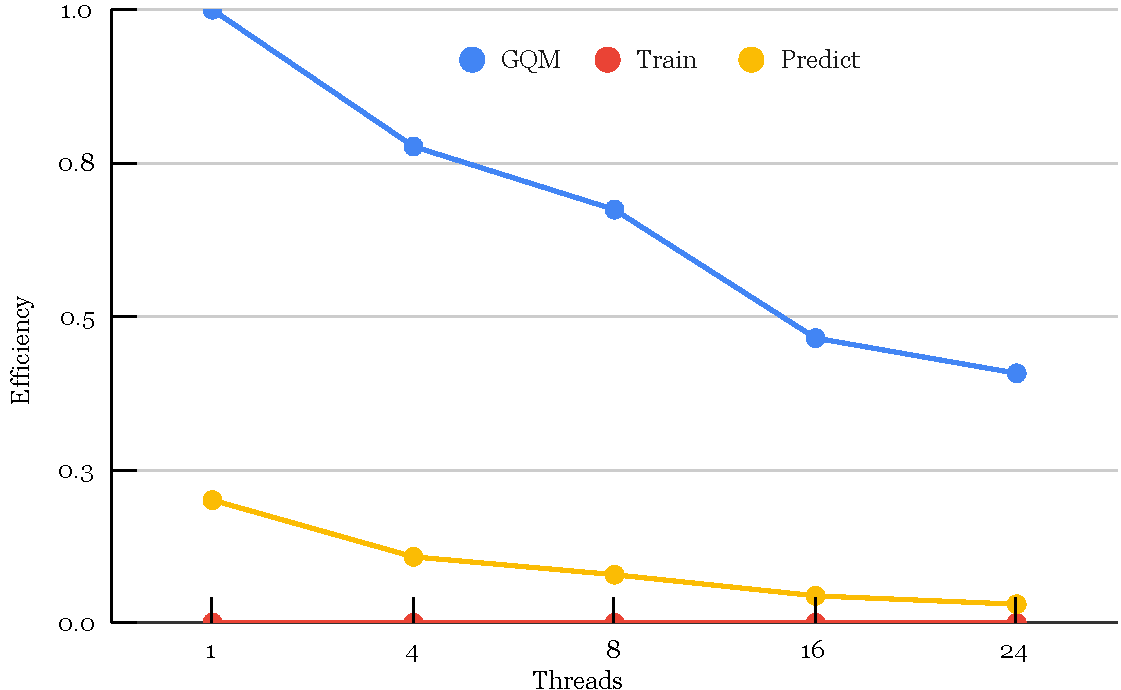
\includegraphics[width=\linewidth]{resu_effi}
\caption{Parallel efficiencies in function of the number of OpenMP threads for the GQM and PINN implementations. "Train" refer to the PINN training phase, while "Predict" refers to the PINN test/prediction phase.}
\label{fig:effi}
\end{figure}

\autoref{tab:resu} shows the processing times for the PINN and GQM solutions. PINN time is splitted into training time (Train) and prediction time (Predict). The singe-thread runtime of the GQM implementation was taken as reference. In all cases, the GQM implementation achieved the best performance, i.e. required less processing times, presented better speedups and parallel efficiencies, even if considering only the PINN prediction time. 

%
%----------------------------------------
\section{Conclusions}\label{sec:conc}
%----------------------------------------
%
This work compares the solutions of a one-dimensional viscous Burgers’ equation of a test problem using a Physics Informed Neural Network (PINN) and a numerical Gaussian Quadrature Method (GQM) method. The Burgers' equation is a partial differential equation (PDE) with derivatives in both space and time, which is commonly solved by a numerical method, as the GQM. A comparison of the accuracy and required processing time of both solutions executed in the LNCC Santos Dumont supercomputer is also presented for different number of OpenMP threads using CPU cores. The GQM presented much lower processing times, and better speedups and parallel efficiencies. As future work, it is intended to exploit other PINN architectures and numerical methods, as well as taking advantage of GPU use, mainly for the PINN.







% The asterisk symbol (*) is used to indicate that a environment does not produce numbering
%----------------------------------------
% \section*{References}
%----------------------------------------
%
\FloatBarrier
\bibliographystyle{IEEEtran}
\bibliography{library.bib}
%
%========================================
\end{document}
%========================================





